\documentclass[12pt, a4paper]{article}
\usepackage[francais]{babel}
\usepackage{caption}
\usepackage{graphicx}
\usepackage[T1]{fontenc}
\usepackage{listings}
\usepackage{geometry}
\usepackage{minted}
\usepackage{array,multirow,makecell}
\usepackage{float}
\usepackage[colorlinks=true,linkcolor=black,anchorcolor=black,citecolor=black,filecolor=black,menucolor=black,runcolor=black,urlcolor=black]{hyperref}
\setcellgapes{1pt}
\makegapedcells
\usepackage{fancyhdr}
\pagestyle{fancy}
\lhead{}
\rhead{}
\chead{}
\rfoot{\thepage}
\lfoot{Baumgaertner - Rehm - Doghmane}
\cfoot{}
\renewcommand{\footrulewidth}{0.4pt}
\renewcommand{\headrulewidth}{0.4pt}
\renewcommand{\listingscaption}{Code}
\renewcommand{\listoflistingscaption}{Table des codes}

% \usepackage{mathpazo} --> Police à utiliser lors de rapports plus sérieux

\begin{document}
\begin{titlepage}
	\newcommand{\HRule}{\rule{\linewidth}{0.5mm}} 
	\center 
	\textsc{\LARGE iut de colmar}\\[4.5cm] 
	\textsc{\Large SAE 24}\\[0.5cm] 
	\textsc{\large projet intégratif}\\[0.5cm]
	\HRule\\[0.75cm]
	{\huge\bfseries Rapport}\\[0.4cm]
	\HRule\\[1.5cm]

	% Utiliser les lignes qui suivent dans le cas où il y a plusieurs membres
	%------------------------------------
	\begin{minipage}{0.4\textwidth}
		\begin{flushleft}
			\large
			\textit{RT11}\\
			Martin \textsc{Baumgaertner}
		\end{flushleft}
	\end{minipage}
	~
	\begin{minipage}{0.4\textwidth}
		\begin{flushright}
			\large
			\textit{RT12}\\
			Mehdi \textsc{Rehm}
		\end{flushright}
	\end{minipage}
    \\[0.7cm]
    \begin{minipage}{0.4\textwidth}
		\begin{flushleft}
			\large
			\textit{RT11}\\
			Sâji \textsc{Doghmane}
		\end{flushleft}
	\end{minipage}
	~
    \begin{minipage}{0.4\textwidth}
		\begin{flushright}
			\large
			\textit{\textcolor{white}{Mehdi}}\\
			\textcolor{white}{Mehdi} \textsc{\textcolor{white}{Mehdi}}
		\end{flushright}
	\end{minipage}
    
	%------------------------------------
    %------------------------------------
	% \textsc{\large martin baumgaertner}\\[0.5cm] % S'il y que moi qui écrit
    %------------------------------------
	\vfill\vfill\vfill
	{\large\today} 
	\vfill
\end{titlepage}
\newpage
\tableofcontents
\newpage
\listoflistings
\newpage
\listoffigures
\newpage

\section*{Introduction}
Nous avons fait face à de nombreuses situations lors de notre première année
universitaire en B.U.T. Réseaux et Télécommunications. Nous avons appris 
par exemple, la gestion de routeurs/switch, en passant par la création de 
VLANs jusqu'à la mise en place d'une topologie réseau.\\ 
Mais aussi, nous avons vu dans les grandes parties ce qu'était la téléphonie
d'entreprise, en configurant des PABX et des téléphones IP, numériques et
analogiques.\\
Pour finir, nous avons pris connaissance de ce qu'était le développement 
web, par l'apprentissage de différents langages de programmation, comme
le HTML, CSS, Python, et Django, qui est un framework python. Les services
MQTT comme la récéption de données envoyés par un capteur de température 
par exemple ont aussi été abordé durant notre année.\\

Toutes ces parties sont donc au sujet de notre dernière SAE, qui fera l'objet
d'une évaluation très importante.\\

Lors de ce projet intégratif nous serons amenés à créer un réseau comprenant
plusieurs parties, pour y déployer plusieurs services. Notamment un serveur 
FTP et Web, une solution de collecte de données, ainsi qu'un PABX
que nous deploierons dans un VLAN spécifique avec le matériel adéquat.
Voici un schéma résumant le réseau que nous allons créer :
\begin{figure}[H]
    \centering
    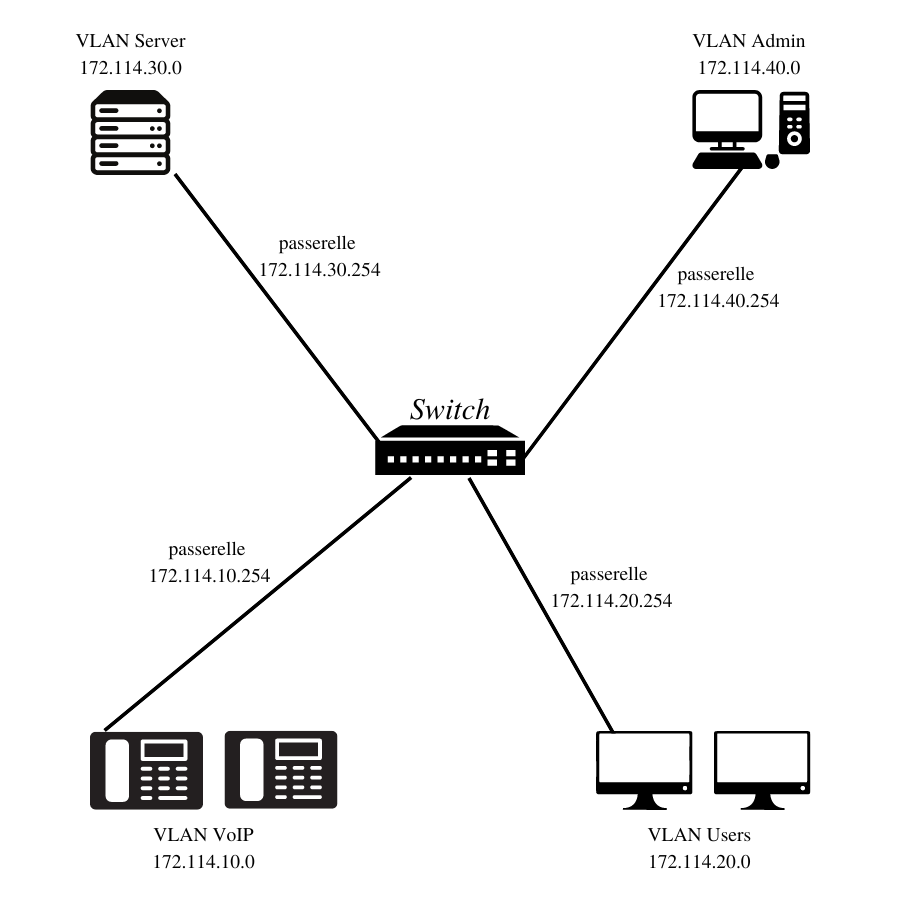
\includegraphics[width=0.5\textwidth]{img/topologie.png}
    \caption{Topologie de notre réseau}
    \label{fig:topologie}
\end{figure}


\newpage
\section{Réseau}
	\subsection{Introduction}
	Dans cette partie nous verrons le commencement de la SAE. Nous allons
	devoir configurer un réseau pour pouvoir y déployer plusieurs services. 
	Nous avons vu sur le schéma précédent que nous serions amener à créer 
	des VLANs, et configurer des access-lists selon les besoin 
	du client. Mais aussi, nous déployerons un serveur FTP et un serveur web
	sur depuis une machine windows server.\\
	Le but de cette partie étant de créer un réseau complet, pour pouvoir
	par la suite faire les autres parties en toute tranquilité.

	\subsection{Création des réseaux}
		\subsubsection{Configuration des VLANs}
		Nous avons donc commencer par créer les VLANs sur le switch.\\
		Pour créer un VLAN, il suffit de rentrer dans les ou l'interface(s) 
		que nous souhaitons affecter à un VLAN, et de lui dire donc quel VLAN
		sera affecté à cette/ces interfaces.\\
		Voici, des captures d'écrans des configurations des VLANs :\\[0.5cm]
		\begin{figure}[h]
			\begin{minipage}[c]{.46\linewidth}
				\centering
				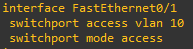
\includegraphics{screens/SW/Interface-VLAN10.png}
				\caption{Interface VLAN10}
			\end{minipage}
			\hfill%
			\begin{minipage}[c]{.46\linewidth}
				\centering
				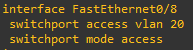
\includegraphics{screens/SW/Interface-VLAN20.png}
				\caption{Interface VLAN20}
			\end{minipage}
		\end{figure}

		\begin{figure}[h]
			\begin{minipage}[c]{.46\linewidth}
				\centering
				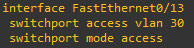
\includegraphics{screens/SW/Interface-VLAN30.png}
				\caption{Interface VLAN30}
			\end{minipage}
			\hfill%
			\begin{minipage}[c]{.46\linewidth}
				\centering
				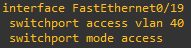
\includegraphics{screens/SW/Interface-VLAN40.png}
				\caption{Interface VLAN40}
			\end{minipage}
		\end{figure}
		\newpage

		\subsubsection{Routage Inter-VLAN}
		Ensuite, pour que nos VLANs puissent communiquer, nous avons mis un
		en place un routage inter-vlans sur le routeur que voici :\\
		\begin{figure}[H]
			\centering
			\includegraphics[width=0.7\textwidth]{screens/routeur/interface.png}
			\caption{Routage Inter-Vlans}
			\label{fig:intervlan}
		\end{figure}

		\subsubsection{Vérification du réseau}

	\subsection{Configuration du NAT}

	\subsection{Mise en place des ACL}

	\subsection{Mise en place des services demandés}

		\subsubsection{Création du serveur FTP}

		\subsubsection{Création du serveur WEB}
	
	\subsection{Vérification des services}




\newpage
\section{Téléphonie}
\subsection{Introduction}


\newpage
\section{Collecte de données}
\subsection{Introduction}
Au courant de l'année nous avons pu voir différents mode de collecte de
données, notamment la récupération via MQTT. D'abord, qu'est-ce que MQTT ?
MQTT, pour "Message Queuing Telemetry Transport", est un protocole
open source de messagerie qui assure des communications non permanentes
entre des appareils par le transport de leurs messages.\\
Le but de cette partie étant de récupérer des données. Nous devons réceptionner
des valeures de température sur une pièce. Nous devons être capable de
les afficher selon les critères définit, et les intégrer dans une base de
données qui nous servira plus tard pour la partie Web. 
	\subsection{Récupération de données}
		\subsubsection{Configuration du script}
		Pour pouvoir récupérer les données depuis le MQTT, j'ai donc dû
		adapter le script python que nous a été donné dans le diaporama
		et j'ai du l'adapter pour qu'il récupère les bonnes données.\\ 
		J'ai modifié les lignes suivantes, en y ajoutant les bonnes valeurs
		de connexion :
		\begin{listing}[H]
			\caption{Configuration des IDs de connexion}
			\label{lst:id}
			\begin{minted}{py}
		broker = 'test.mosquitto.org'
		topic = "IUT/Colmar/SAE24/Maison1"
			\end{minted}
		\end{listing}
		Par la suite j'ai du installer un paquet qui était prérequis 
		pour que le script puisse s'éxecuter correctement à savoir :
		\begin{listing}[H]
			\caption{Installation des paquets nécessaire au script MQTT}
			\label{lst:paho}
			\begin{minted}{bash}
		pip3 install paho-mqtt python-etcd
			\end{minted}
		\end{listing}
		\newpage
		\subsubsection{Éxécution du script}
		Au moment de l'éxécution du programme, j'obtiens bien les valeurs que 
		nous voulions recevoir comme nous pouvons le constater ci dessous :
		\begin{figure}[H]
			\centering
			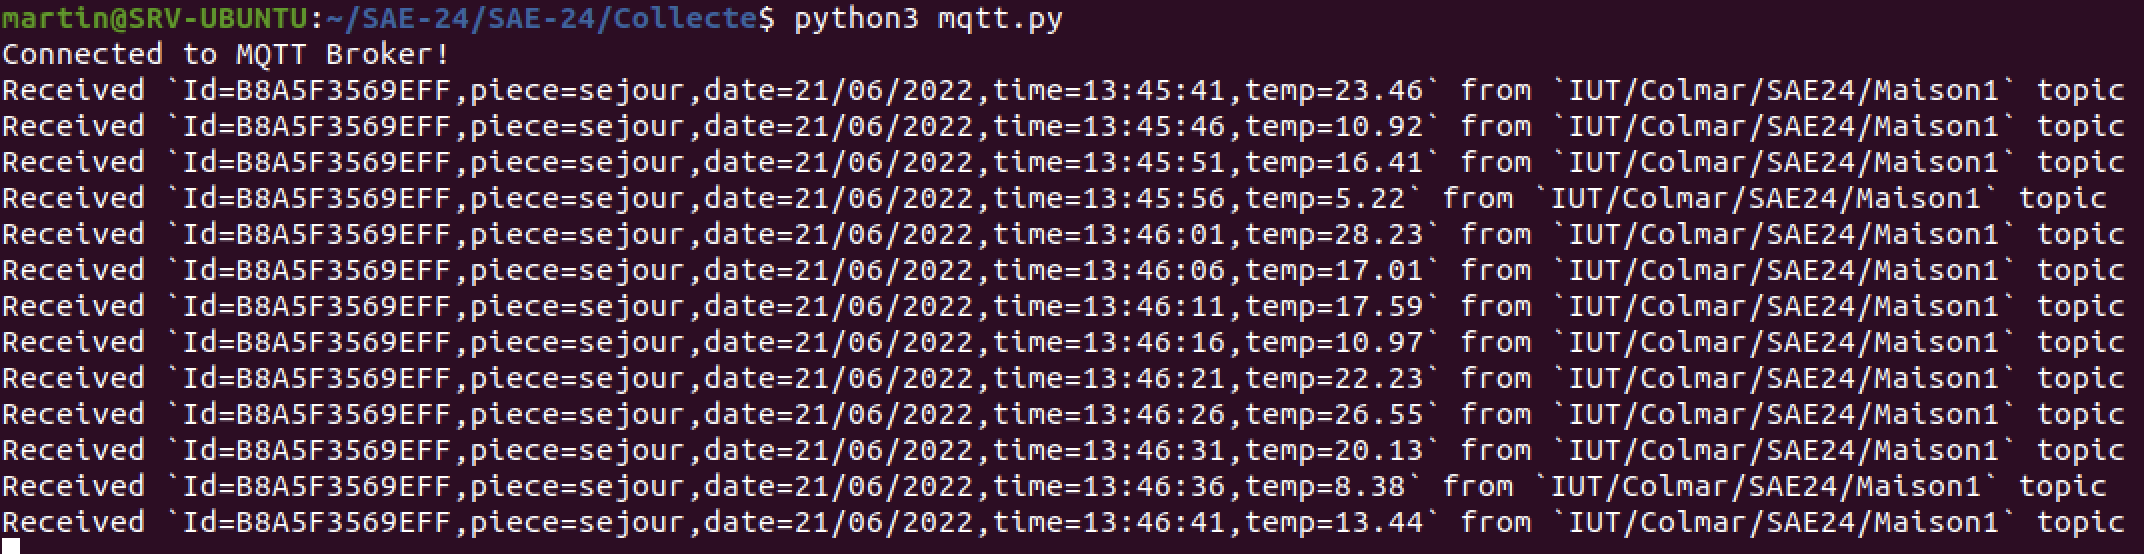
\includegraphics[width=1\textwidth]{img/recup.png}
			\caption{Récupération des données}
			\label{fig:recup}
		\end{figure}
		Le problème est qu'il nous était demandé de récupérer un ID différent
		à chaque fois qu'une valeur de température est reçue.

	\subsection{Sauvegarde des valeurs dans la base de données}


\newpage
\section{Web/Base de données}
\subsection{Introduction}


\end{document}